\chapter{Heisenbergsche Unsch"arferelation\label{chapter:heisenberg}}
\lhead{Heisenbergsche Unsch"arferelation}
\rhead{}

In der Quantenmechanik lassen sich die Observablen nicht mehr einfach
vertauschen, wie das in der klassischen Mechanik m"oglich war.
F"ur Operatoren gilt im Allgemeinen kein Kommutativgesetz.
In diesem Abschnitt wollen wir die Konsequenzen dieser Tatsache
untersuchen.
Wir k"onnen aber bereits jetzt feststellen, dass die Gleichung
$AB=BA$ f"ur zwei quantenmechanische Observable ``fast'' stimmen
muss, in dem Sinne, dass der Unterschied der beiden Seiten sehr
klein sein muss. 

\section{Kommutator und Antikommutator}
\rhead{Kommutator und Antikommutator}
\index{Kommutator}
\index{Antikommutator}
Zu zwei Operatoren $A$ und $B$ kann man Kommutator und Antikommutator
bilden:
\[
\begin{aligned}
&\text{Kommutator:}&
[A,B]&=AB-BA
\\
&\text{Antikommutator:}&
\{A,B\}&=AB+BA
\end{aligned}
\]
Wenn $[A,B]=AB-BA=0$ folgt $AB=BA$,
der Kommutator gibt also an, ob die beiden Operatoren vertauschen (kommutieren).
Wenn $\{A,B\}=AB+BA=0$ folgt $AB=-BA$,
der Kommutator gibt also an, ob die beiden Operatoren antikommutieren.

Falls $A$ and $B$ Observable sind, die nicht vertauschen, dann k"onnen
gemeinsame Eigenvektoren nicht beliebig sein.
Nehmen wir n"amlich an, $|\psi\rangle$ sei ein gemeinsamer Eigenvektor
von $A$ mit Eigenwert $\alpha$ und $B$ mit Eigenwert $\beta$.
Dann wirkt der Kommutator auf $|\psi\rangle$ wie folgt
\[
[A,B]\,|\psi\rangle
=
(AB-BA)\,|\psi\rangle 
=
A\beta\,|\psi\rangle -B\alpha\,|\psi\rangle
=
\alpha\beta\,|\psi\rangle-\beta\alpha\,|\psi\rangle
=
0.
\]
Ein gemeinsamer Eigenvektor $|\psi\rangle$ wird also von $[A,B]$
zu $0$ gemacht.

F"ur die Observablen $X$ f"ur Ort und $P$ f"ur den Impuls eines Teilchens,
k"onnen wir den Kommutator in der Ortsdarstellung explizt ausrechnen:
\begin{align*}
[X,P]\psi(x)
&=
\biggl[
x,\frac{\hbar}{i}\frac{\partial}{\partial x}
\biggr]\psi(x)
=
x\frac{\hbar}{i}\frac{\partial\psi(x)}{\partial x}
-
\frac{\hbar}{i}\frac{\partial}{\partial x}\bigl(x\psi(x)\bigr)
\\
&=
x\frac{\hbar}{i}\frac{\partial\psi(x)}{\partial x}
-
\frac{\hbar}{i}\psi(x)
-
\frac{\hbar}{i}x\frac{\partial\psi(x)}{\partial x}
=
-\frac{\hbar}{i}\psi(x).
\end{align*}
Der Kommutator ist also
\[
[X,P]=-\frac{\hbar}{i}\operatorname{id},
\]
ein Vielfaches der identischen Abbildung.
Die identische Abbildung hat nat"urlich keine Vektoren, die von ihr
zu $0$ gemacht werden.
Orts- und Impuls-Operatoren k"onnen also keine gemeinsamen Eigenvektoren
haben.
Es gibt also keinen Zustand, in dem sowohl Ort als auch Impuls exakt
bestimmt sind.

\begin{satz}
Wenn zwei Observable einen Kommutator haben, der ein Vielfaches
der identischen Abbildung ist, dann haben die Observable keine
gemeinsamen Eigenvektoren.
Insbesondere k"onnen die beiden Observablen nicht gleichzeitig 
exakt bestimmt sein.
\end{satz}

In der klassischen Mechanik haben wir keine Schwierigkeit, Ort und
Impuls gleichzeitig festzustellen. Das liegt nat"urlich daran, dass
der Kommutator den sehr kleinen Faktor $\hbar$ enth"alt.
F"ur makroskopische Zwecke sind Ort und Impuls also gleichzeitig 
feststellbar.

Wenn es also nicht m"oglich ist, Ort und Impuls eines Teilchens
gleichzeitig exakt zu wissen, wie genau ist es dann m"oglich,
Ort und Impuls zu wissen?
Um diese Frage zu beantworten m"ussen wir zun"achst ein Mass f"ur
die Genauigkeit finden, mit der Ort oder Impuls in einem bestimmten
Zustand bekannt sein kann.
Wir werden es die Unsch"arfe nennen.
Wir erwarten dann eine Ungleichung, die uns sagt, wie grosse 
Unsch"arfe sein muss, eine Unsch"arferelation.


\section{Varianz, Kovarianz und Unsch"arfe}
\rhead{Varianz, Kovarianz und Unsch"arfe}
Sie $A$ eine Observable und $|\psi\rangle$ ein Zustand. Dann ist
$\langle \psi|\,A\,|\psi\rangle$ der Erwartungswert der Observablen $A$ 
im Zustand $|\psi\rangle$.
Zur Abk"urzung schreiben wir $\langle A\rangle=\langle\psi|\,A\,|\psi\rangle$.
Mit $A$ ist auch $A-\langle A\rangle$ eine Observable, und ihr Erwartungswert
ist nat"urlich $0$.

In der Wahrscheinlichkeitsrechnung lernt man mit der Varianz eine
Gr"osse kennen, die angibt, wie nahe bei $\langle A\rangle$ die
Werte der Observable im Mittel anzutreffen sind.
Die Varianz ist die mittlere quadratische Abweichung, also der
Erwartungswert der Gr"osse $(A-\langle A\rangle)^2$, die auch wieder
eine Observable ist. Sie kann also mit unserem Formalismus berechnet
werden:
\begin{align*}
\operatorname{var}(A)
&=
\langle \psi|\, (A-\langle A\rangle)^2\,|\psi\rangle
=
\langle\psi|\, A^2-2\langle A\rangle A+\langle A\rangle^2\,|\psi\rangle
=
\langle\psi|\,A^2\,|\psi\rangle 
-2\langle A\rangle \langle\psi|\,A\,|\psi\rangle
+\langle A\rangle^2\langle\psi|\psi\rangle
\\
&=\langle A^2\rangle -\langle A\rangle^2.
\end{align*}
Dies entspricht der aus der Wahrscheinlichkeitsrechung bekannten Formel
$E(X^2)-E(X)^2$.
Wir nennen die Standardabweichung, also
\[
\sqrt{\operatorname{var}(A)}
=
\sqrt{\langle (A-\langle A\rangle)^2\rangle}
=
\sqrt{\langle A^2\rangle - \langle A\rangle^2}
\]
auch die {\em Unsch"arfe} der Messung von $A$, und schreiben daf"ur abgek"urzt
auch $\Delta A$.

Die Varianz ist ein Spezialfall der Kovarianz, die als 
\[
\operatorname{cov}(X,Y)
=
E((X-E(X))(Y-E(Y)))
\]
definiert war, $\operatorname{var}(X)=\operatorname{cov}(X,X)$.
Analog k"onnen wir jetzt auch eine Kovarianz f"ur Observable als
\[
\langle A,B\rangle
=
\langle\psi|
\,
(A-\langle A\rangle)(B-\langle B\rangle)
\,
|\psi\rangle
\]
definieren.
Man beachte, dass die Gr"osse $\langle A,B\rangle$ nicht symmetrisch zu
sein braucht, ausser wenn die Operatoren $A$ und $B$ vertauscht werden
k"onnen.

Man kann $\langle A,B\rangle$ auch als den Wert der Transformationsfunktion 
zweier Zust"ande ansehen:
\begin{equation}
\left.
\begin{aligned}
|a\rangle &= (A-\langle A\rangle)\,|\psi\rangle\\
|b\rangle &= (B-\langle B\rangle)\,|\psi\rangle
\end{aligned}
\right\}
\quad
\Rightarrow
\quad
\langle A,B\rangle = \langle a|b\rangle.
\end{equation}
Nat"urlich gilt die Cauchy-Schwarz-Ungleichung f"ur die beiden
Zust"ande $|a\rangle$ und $|b\rangle$, also
\begin{equation}
|\langle a|b\rangle|^2
\le
\langle a|a\rangle \langle b|b\rangle
=
\operatorname{var}(A)\operatorname{var}(B)
=\Delta A^2 \cdot \Delta B^2
\label{skript:cauchy-schwarz-uncertainty}
\end{equation}
Falls also die linke Seite nicht $0$ ist, dann k"onnen wir die beiden
Gr"ossen $A$ und $B$ nicht beliebig genau kennen.
Die Ungenauigkeit, mit der $A$ und $B$ bekannt sein k"onnen, sind "uber
die Ungleichung (\ref{skript:cauchy-schwarz-uncertainty}) miteinander verkn"upft.
Wenn die Unsch"arfe verkleinert wird, mit der $A$ bekannt ist, dann 
vergr"ossert sich die Unsch"arfe, mit der $B$ bekannt ist.

Um das Unsch"arfeprodukt nach unten absch"atzen zu k"onnen, m"ussen
wir $\langle a|b\rangle$ ausrechnen:
\begin{align}
\langle a|b\rangle
&=
\langle\psi|\,
(A-\langle A\rangle)(B-\langle B\rangle)
\,|\psi\rangle
=
\langle\psi|\,
AB-\langle A\rangle B-A\langle B\rangle
+
\langle A\rangle\langle B\rangle
\,|\psi\rangle
\notag
\\
&=
\langle\psi|\,AB\,|\psi\rangle
-\langle B\rangle\langle\psi|\,A\,|\psi\rangle
-\langle A\rangle\langle\psi|\,B\,|\psi\rangle
+
\langle A\rangle\langle B\rangle
\notag
\\
&=
\langle\psi|\,AB\,|\psi\rangle
-
\langle A\rangle\langle B\rangle.
\label{skript:abausrechnung}
\end{align}

%
% Unschaerferelation
%
\section{Unsch"arferelation}
\rhead{Unsch"arferelation}
\begin{figure}
\centering
\includegraphics{graphics/heisenberg-1.pdf}
\caption{Einstein-Podolsky-Rosen Experiment
\label{skript:epr-experiment}}
\end{figure}
Werner Heisenberg hat 1926 eine Unsch"arferelation zwischen Ort und Impuls
mit Hilfe eines klassischen Gedankenexperimentes hergeleitet.
Seine Erkl"arung beruht auf dem Beobachter-Effekt: jede Messung
ver"andert das beobachtete System.
\index{Einstein-Podolsky-Rosen Experiment}
Der Beobachter-Effekt reicht jedoch f"ur die Begr"undung nicht
aus, wie man aus dem folgenden Gedanken-Experiment von Einstein,
Podolsky und Rosen sehen kann, siehe
auch Abbildung~\ref{skript:epr-experiment}, \cite{skript:epr}.
In diesem Experiment werden im Nullpunkt aus einem ruhenden System
zwei Teilchen ausgesandt.
Da der Impuls erhalten ist, m"ussen die Teilchen exakt entgegengesetzen
Impuls haben.
Wenn man nach einer bestimmten Zeit die Position des linken Teilchens misst,
weiss man auch die Position des rechten Teilchens.
Und wenn man den Impuls des rechten Teilchens misst, dann weiss
man auch den Impuls des linken Teilchens.
Es scheint, dass man mit dieser Apparatur Heisenbergs Unsch"arferelation
umgehen kann.
Offenbar braucht es eine bessere Begr"undung f"ur die Unsch"arferelation.

\subsection{Robertson-Schr"odinger-Unsch"arferelation}
\index{Robertson-Schr\"odinger-Unsch\"arferelation}
Die Ungleichung (\ref{skript:cauchy-schwarz-uncertainty}) liefert eine
Unsch"arferelation, falls die linke Seite $>0$ ist. Es ist
also zu untersuchen, wie gross die linke Seite von 
(\ref{skript:cauchy-schwarz-uncertainty}) tats"achlich ist.
Setzen wir $z=\langle a|b\rangle$, dann ist $|z|^2$ die linke Seite
von (\ref{skript:cauchy-schwarz-uncertainty}). Den Betrag kann man mit Hilfe
von Real- und Imagin"arteil unter Zuhilfenahme von (\ref{skript:abausrechnung})
ausrechnen:
\[
|z|^2
=
(\operatorname{Re}z)^2+(\operatorname{Im}z)^2
=
\biggl(\frac{z+\bar z}2\biggr)^2 + \biggl(\frac{z-\bar z}{2i}\biggr)^2
\]
(Vergleiche hierzu auch die Formeln (\ref{skript:realteil-formel}) und 
(\ref{skript:imaginaerteil-formel})).
Jetzt setzen wir $z=\langle a|b\rangle$ ein:
\begin{equation}
|\langle a|b\rangle|^2
=
\biggl(\frac{\langle a|b\rangle + \langle b|a\rangle}2\biggr)^2
+
\biggl(\frac{\langle a|b\rangle - \langle b|a\rangle}{2i}\biggr)^2
\label{skript:unschaerfe2}
\end{equation}
Wir m"ussen also die Terme $\langle a|b\rangle + \langle b|a\rangle$
und $\langle a|b\rangle - \langle b|a\rangle$ ausrechnen:
\begin{align*}
\frac{\langle a|b\rangle + \langle b|a\rangle}2
&=
\frac{
\langle\psi|AB+BA|\psi\rangle 
}2
-\langle A\rangle\langle B\rangle
=
\frac12 \langle\,\{A,B\}\,\rangle - \langle A\rangle\langle B\rangle,
\\
\frac{\langle a|b\rangle - \langle b|a\rangle}{2i}
&=
\frac{\langle\psi|AB-BA|\psi\rangle}{2i}
=
\frac1{2i}\langle [A,B]\rangle
\end{align*}
Eingesetzt in (\ref{skript:unschaerfe2}) finden wir
\[
|\langle a|b\rangle|^2
=
\biggl(
\frac12\langle \{A,B\}\rangle - \langle A\rangle\langle B\rangle
\biggr)^2
+
\biggl(
\frac{\langle[A,B]\rangle}{2i}
\biggr)^2.
\]
Eingesetzt in die urspr"ungliche Unsch"arferelation
(\ref{skript:cauchy-schwarz-uncertainty}) erhalten wir jetzt die Unsch"arferelation
von Robertson und Schr"odinger:

\begin{satz}
\label{skript:robertson-schroedinger-unschaerfe}
Sind $A$ und $B$ selbstadjungierte Operatoren und $|\psi\rangle$ ein
Zustand, dann gilt die Unsch"arferelation
\begin{equation}
\Delta A^2\cdot\Delta B^2\ge 
\biggl(
\frac12\langle \{A,B\}\rangle - \langle A\rangle\langle B\rangle
\biggr)^2
+
\biggl(
\frac{\langle[A,B]\rangle}{2i}
\biggr)^2.
\label{skript:uncertainty}
\end{equation}
\end{satz}

F"ur Ort und Impuls haben wir den Kommutator schon ausgerechnet, es
muss also gelten
\begin{equation}
\Delta X^2\cdot \Delta P^2
\ge
\biggl(
\frac12\langle \{X,P\}\rangle - \langle X\rangle\langle P\rangle
\biggr)^2
+
\biggl(
\frac{\langle[X,P]\rangle}{2i}
\biggr)^2
\ge
\biggl(
\frac{\langle[X,P]\rangle}{2i}
\biggr)^2
\ge \frac{\hbar^2}4
\end{equation}
oder
\begin{equation}
\Delta X\cdot\Delta P\ge \frac{\hbar}2.
\end{equation}
Dies ist die Heisenbergsche Unsch"arferelation. 

\subsection{Drehimpuls und Positionswinkel}
Heisenberg-Unsch"arfe war auch schon Thema bei XKCD, siehe
Abbildung~\ref{skript:heisenberg:xkcd} und \cite{skript:xkcd}.
\begin{figure}
\centering
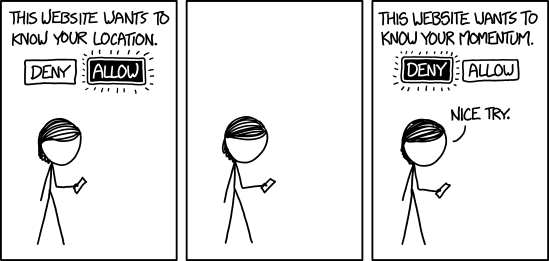
\includegraphics[width=0.8\hsize]{images/xkcd-location-sharing.png}
\caption{XKCD Comic zur Heisenberg Unsch"arfe. Die Benutzerin stellt sicher,
dass die Heisenbergsche Unsch"arferelation nicht verletzt wird. Man kann nicht
sowohl den Ort als auch den Impuls wissen.
\label{skript:heisenberg:xkcd}}
\end{figure}
Im Kapitel~\ref{chapter:drehimpuls} werden wir ein weiteres Paar
von Operatoren wie Ort und Impuls kennen lernen.
Dort untersuchen wir die Komponente $L_3$ des Drehimpulses in $z$-Richtung.
Die dazugeh"orige Ortskoordinaten ist in Kugelkoordinaten die geographische 
L"ange $\varphi$ des Teilchens, welche durch eine Observable mit Operator
$\Phi$ festgestellt werden kann.
In Kugelkoordinaten hat $L_3$ die Form
\[
L_3=\frac{\hbar}{i}\frac{\partial}{\partial\varphi}.
\]
Die Vertauschungsrelationen f"ur $\Phi$ und $L_3$ sind
\[
[\Phi,L_3]=\frac{\hbar}{i}\operatorname{id},
\]
das entspricht den Vertauschungsrelationen von $X$ und $P$.
Zu $\Phi$ und $L_3$ geh"ort nach Satz~\ref{skript:robertson-schroedinger-unschaerfe}
die Unsch"arferelation
\[
\Delta\varphi\cdot\Delta l_3 \ge \frac{\hbar}2,
\]
man kann also den Drehimpuls und die Richtung $\varphi$ nicht gleichzeitig
beliebig genau kennen.
Dies erkl"art den Mouse-Over-Text des Comics in
Abbildung~\ref{skript:heisenberg:xkcd}:
\begin{quote}
Our phones must have great angular momentum sensors because
the compasses really suck.
\end{quote}

\subsection{Unsch"arfe von Energie und Zeit}
In unserem Formalismus hat die Zeit-Koordinate eine ausgezeichnete
Bedeutung, die Schr"odingergleichung beschreibt die Entwicklung
der Zust"ande in der Ortsdarstellung.
Dies hat zur Folge, das wir eine Unsch"arferelation zwischen Energie
und Zeit nicht aus der Robertson-Schr"odinger-Unsch"arferelation
(\ref{skript:uncertainty}) herleiten k"onnen.

Dazu br"auchten wir eine Theorie, welche Orts- und Zeitkoordinaten
gleichwertig behandelt.
Eine solche Theorie ist die spezielle Relativit"atstheorie, welche
zeigt, wie Raum und Zeit untrennbar in einer vierdimensionalen
Raumzeit miteinander verbunden sind.

F"ur einen Spezialfall kann man eine Unsch"arferelation zwischen
Energie und Zeit finden.
Betrachten wir dazu ein Photon mit Energie $E=h\nu$.
Schon die klassische Elektrodynamik erkl"art das Ph"anomen des
Strahlungsdrucks, welches auch schon von Raumfahrzeugen ausgenutzt
werden ist, um durch das Sonnensystem zu `segeln'.
Strahlungsdruck bedeutet, dass Photonen Impuls $p=E/c$ transportieren
und "ubertragen.
Da alle Photonen gleich schnell sind, n"amlich $c$, ist die
Positionsunsch"arfe $\Delta x$ eines Photons im Wesentlichen die
Zeitunsch"arfe der Messung $\Delta t$.
Die Heisenbergsche Unsch"arferelation wird daher
\[
\frac{\hbar}2\le \Delta x\cdot\Delta p=c\Delta t\cdot \frac{\Delta E}{c}=
\Delta t\cdot \Delta E.
\]
Die Unsch"arfe zwischen Zeit und Energie bedeutet, dass die
Energieerhaltung um den Betrag $\Delta E$ verletzt werden darf,
wenn auch nur f"ur kurze Zeit $\Delta t$.

\section*{"Ubungsaufgaben}
\rhead{"Ubungsaufgaben}
\begin{uebungsaufgaben}
\item
\input uebungsaufgaben/07001.tex
\item
\input uebungsaufgaben/07002.tex
\item
\input uebungsaufgaben/07003.tex
\end{uebungsaufgaben}
